\section{Medical Visualization System}

As our original goal was to use an existing application and enhance it with certain abilities we researched the web to find open source applications that are cross platform and run under Windows and Linux environments.
As this is a quite restrictive approach we actually found a lot more applications and frameworks but exclude them for the reasons above.

Our search continued then with frameworks as we saw that there was no application that fulfilled our needs and was capable for rapid prototyping our system.
With frameworks we unfortunately also didn't have more luck as the way the frameworks limit us in regards of data import and data visualization was as well not suitable to develop our chosen algoritm rapidly.

In the end we utilize an OpenGL based visualion project to implement our algorithm there. Additional libraries to load DICOM data were searched but also there we experience several problems with codecs for instance.

%\section{Applications}
%
%% Surface Visualization Apps?

\subsection{3DSlicer}

\blockquote{3D Slicer is an open source software platform for medical image informatics, image processing, and three-dimensional visualization \cite{3DSlicer_2018}.}

The power of 3DSlicer lies in the handy user interface and the amount of resources how to deal with the program. Also youtube is a good source and this is how we lernt to do some basic tasks with 3DSlicer. It can also import several kinds of DICOM data, which is a prerequisite for our medical visualization application.

Although very nice at user level we do not discover a developer guide that assists us well through the internals of 3DSlicer.
As our goal was not to use the application but rather to implement renderers for example we hadn't the impression that this would be possible in reasonable amount of time.

%\subsubsection{\emph{MAGIX} Dataset in 3DSlicer}

\begin{figure}[h]
	\centering
	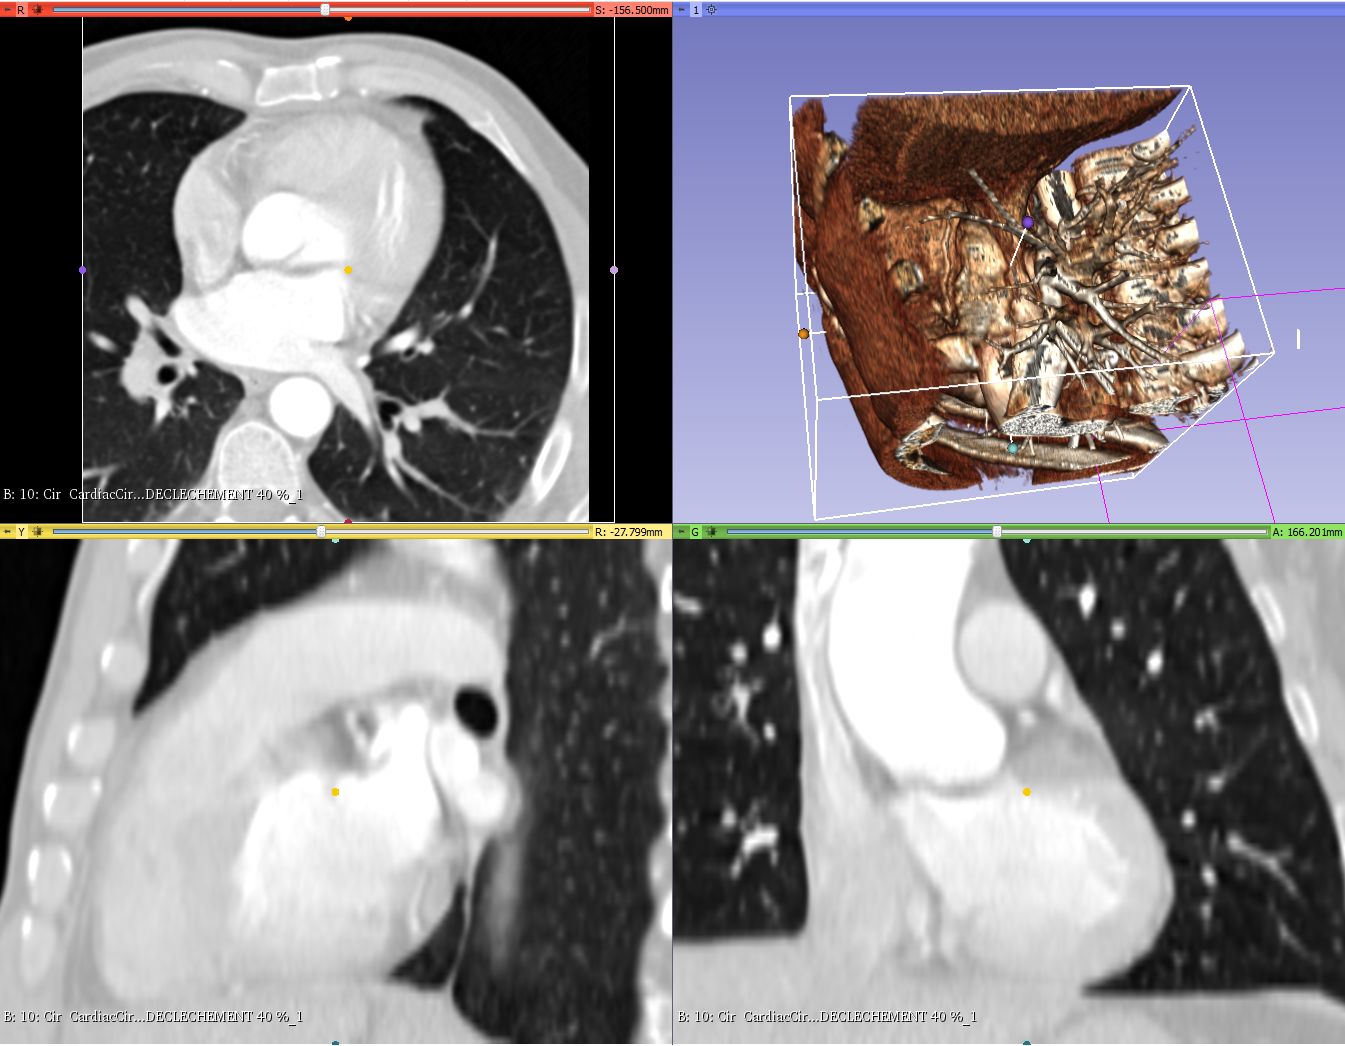
\includegraphics[width=0.45\textwidth]{Slicer3D_MAGIX_01.png} \\
	\caption{ \emph{MAGIX}\cite{gimias_sampledata_2018} dataset visualized with \emph{Slicer3D}.}
	\label{fig:Slicer3D_MAGIX_01}
\end{figure}

As could be seen in figure \ref{fig:Slicer3D_MAGIX_01}, we visualized one of our example datasets, \emph{MAGIX} with volume rendering provided by 3DSlicer.


\subsection{MITK - The Medical Imaging Interaction Toolkit}

\blockquote{The Medical Imaging Interaction Toolkit (MITK) is a free open-source software system for development of interactive medical image processing software. MITK combines the Insight Toolkit (ITK) and the Visualization Toolkit (VTK) with an application framework \cite{MITK_2018}.}

In comparison to 3DSlicer MITK offers a better developer documentation and a description of the internal structure of MITK. Further it supplies guides how to create plugins or template based-projects that help to develop own applications with the MITK framework. Build instructions and a description of the render concept concludes our decision to take a closer look at this open source project.
Also DICOM loaders are integrated and we managed to visualize one of our demo datasets in MITK. A downside was the stability of MITK as it happened several times that the application crashed after selecting DICOM data for volumetric visualization.

% TODO: add ref to chapter
As we are interested in writing an own renderer and as MITK uses VTK to visualize data, we refer here to the VTK section that describes our experience with VTK in more detai.

%\subsubsection{MITK Plugin}

%\subsubsection{\emph{CARDIX} Dataset in MITK}

\begin{figure}[h]
	\centering
	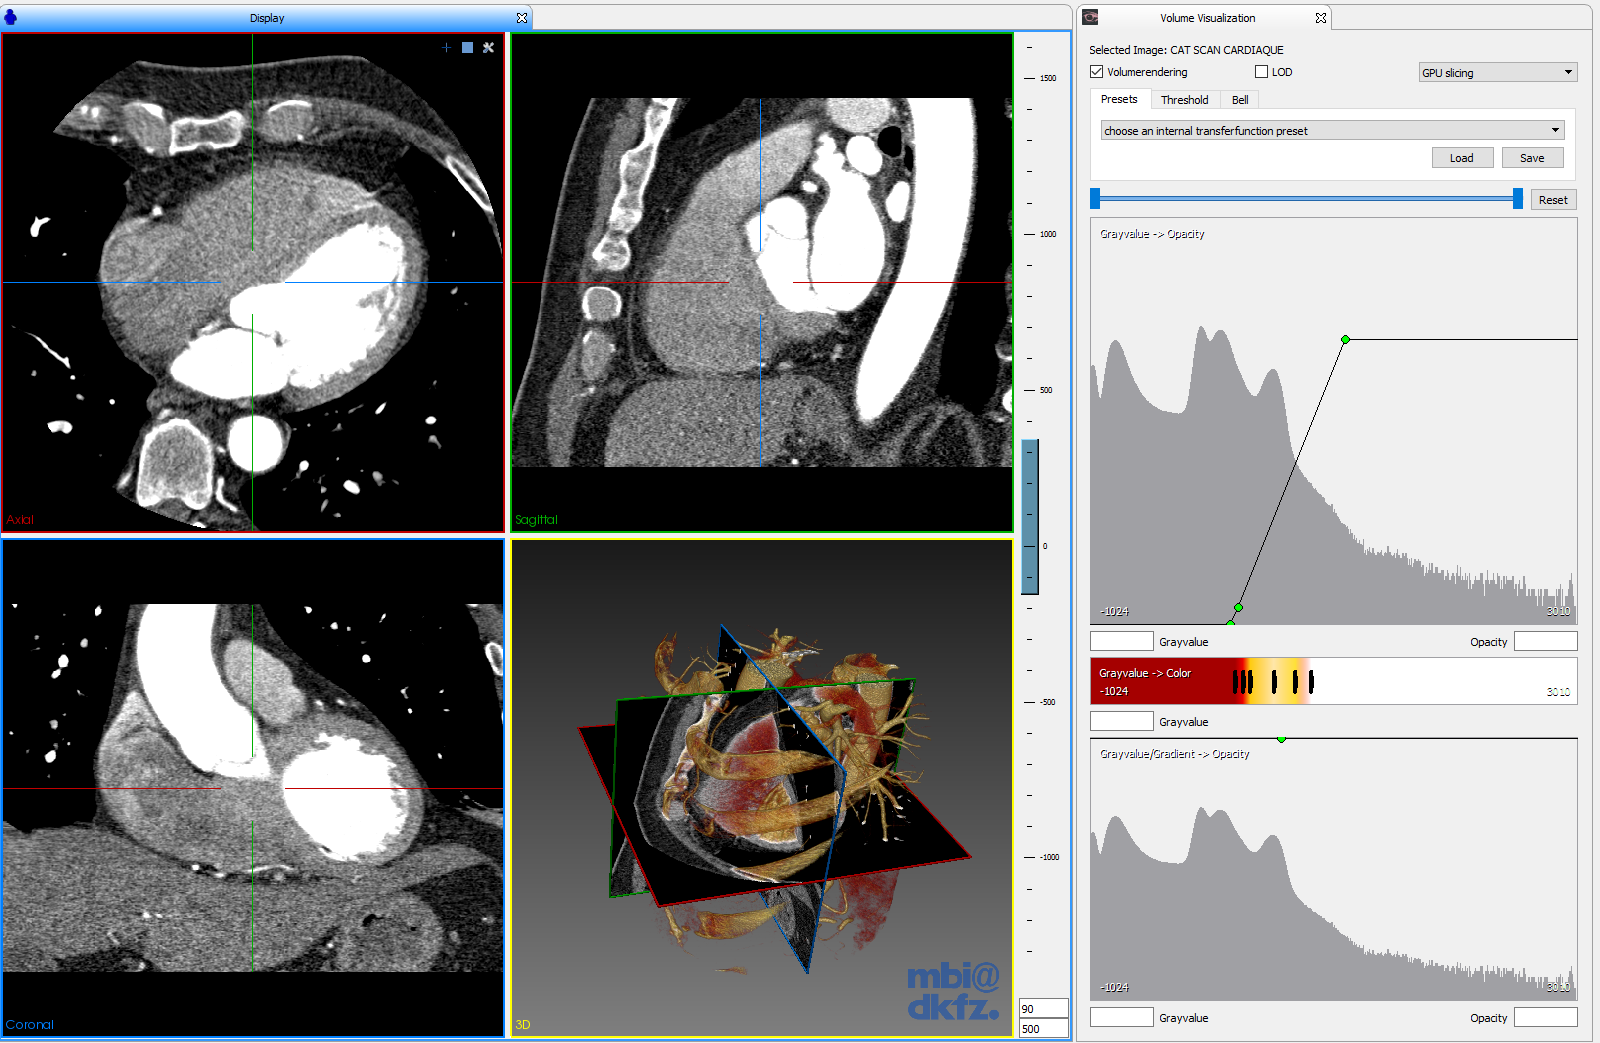
\includegraphics[width=0.45\textwidth]{MITK_CARDIX_01.png} \\
	\caption{ \emph{CARDIX}\cite{gimias_sampledata_2018} dataset visualized with \emph{MITK}.}
	\label{fig:MITK_CARDIX_01}
\end{figure}

As could be seen in figure \ref{fig:MITK_CARDIX_01}, we visualized one of our example datasets, \emph{CARDIX} with volume rendering provided by the MITK application.

%\section{Frameworks}

\subsection{VTK - The Visualization Toolkit}

\blockquote{The Visualization Toolkit (VTK) is an open-source, freely available software system for 3D computer graphics, image processing, and visualization. It consists of a C++ class library and several interpreted interface layers including Tcl/Tk, Java, and Python. VTK supports a wide variety of visualization algorithms including scalar, vector, tensor, texture, and volumetric methods, as well as advanced modeling techniques such as implicit modeling, polygon reduction, mesh smoothing, cutting, contouring, and Delaunay triangulation. VTK has an extensive information visualization framework and a suite of 3D interaction widgets \cite{vtk_2018}.}

As VTK was the central part of actual all medical visualization toolkits researched we wanted to use this framework for our application.
Our resources for learning VTK were \emph{The Visualization Toolkit}\cite{schroeder2004visualization}, \emph{The VTK Users's Guide}\cite{avila2010vtk} and of course the VTK webpage \cite{vtk_2018}.

Several parts of the VTK chain were researched, as there are:

\subsubsection{Loading Data with VTK Readers}
%\subsubsection{VTK Reader}

VTK also supports to load DICOM data via specific VTK Readers. As our data is formed of DICOM files we take a closer look at that feature. Unfortunately due to problems with the codec included in our DICOM data we were not able to load the data as we want to. As we haven't found a solution to fix this we come up with a preconversion step of DICOM data with MITK, as there it is possible to save DICOM data into a VTK 3D image.  


\subsubsection{Processing Data with VTK Filters}

The VTK way of processing data is through VTK Filters. The philosophy is that filters transform or combine data within a chain or network of coupled filters that finally provide an output to one or more VTK Mappers.
To implement our direct volume rendering approach the only easy way would have been to dynamically adapt our DICOM data according to the settings of MIDA and the current view direction and further use a built-in volume renderer like RayCast Mapper to visualize the result.
As we would have to implement somehow a reverse version of MIDA and as the data transformation would have been a seperate step in the processing chain we decided not to use VTK Filters at all.

\subsubsection{Render Data with VTK Mappers}

In VTK renderer are called Mappers as they provide the ability to map a given dataset to a given device. While it is possible to override specific Mappers it is not straight forward to interfere with the renderer at OpenGL-level. 

For this reason VTK introduced VTK shaders, that are based on structured OpenGL shaders. While this give access to GLSL shaders the structure of the shaders have to follow the VTK guidelines. That include string replacement of VTK specific shading commands within the OpenGL shader.

As we haven't found appropriate information on what for string replacements exist, how they should be used and how they interact with the rest of the VTK application we decided not to use an OpenGL shader based on the VTK framework.

\subsubsection{VTK Example Application}

\begin{figure}[h]
	\centering
	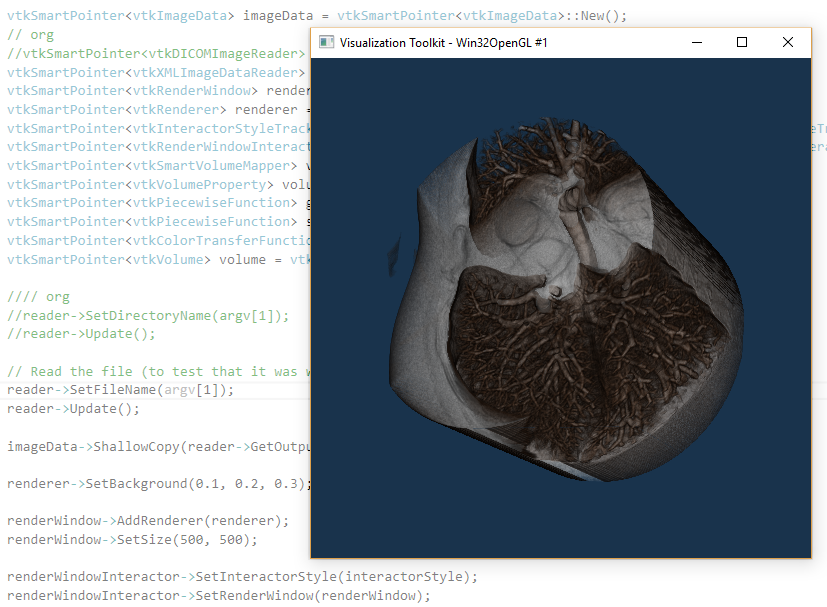
\includegraphics[width=0.45\textwidth]{VTK_Image_Renderer_02_II.png} \\
	\caption{ \emph{CARDIX} \cite{gimias_sampledata_2018} dataset rendered from VTI file with VTK Raycast Mapper.}
	\label{fig:VTK_Image_Renderer_02_II}
\end{figure}

As VTK prodides a lot of examples and tutorials on the usage of its framework we gave it a try and load a 3D image in form of a VTI file into a simple raycaster visualization. In figure \ref{fig:VTK_Image_Renderer_02_II} we see the \emph{CARDIX} \cite{gimias_sampledata_2018} dataset visualized with this base fazilities. As VTK also provide a script interface we also build $Tcl/Tk$ and tried the same visualization on a script base, which works perfectly fine. But as already stated before we left VTK behind as it does not support an easy integration of own OpenGL shaders.

%\subsection{MITK Plugin}

%\section{Library}

% Surface Visualization Libs ?

%\subsection{DICOM Reader}

\subsection{Imbera DICOM Reader}

%Imebra: a C++ Dicom library

\blockquote{Imebra SDK is an open source C++ library that handles DICOM network messages and DICOM files \cite{imebra_dicom_sdk_2018}.}

While Imbera seems to be the library we searched for to easily read DICOM data on multiple platforms in practice it fails because of the codec used in our \emph{CARDIX} dataset. We don't know if this is due to the open source version used as we haven't tried the commercial version instead and will leave this as an open point.

%\subsection{VTK Reader}

\subsection{OpenGL Application}

As stated before we considered using the VTK (Visualization ToolKit) framework as well as the MITK (Medical Imaging Interaction Toolkit) framework. However we soon realized that it is hard to implement a custom volume renderer in these frameworks, and thus decided to fall back to our own implementation. For this we reused an old Qt framework from the vis1 course that had simple GPU direct volume rendering implemented with simple alpha compositing, but with no proper interaction, no transfer functions and no shading.

The goal was to extend this framework with
\begin{itemize}
	\item More compositing methods: Maximum Intensity Projection (MIP), Minimum Intensity Projection (MINIP), Average Intensity Projection (AIP) as well as Maximum Intensity Difference Accumulation (MIDA)
	\item Interactive controls
	\item Gradient-based shading
	\item Customizable transfer functions
\end{itemize}

%\section{MIDA Processing Chain}

% Surface Visualization Chain ?
% MIDA Chain
% To process our data with MIDA we utilize VTK and use its VTI ...

%\section{MIDA Algorithm}

\section{MIDA  - Maximum Intensity Difference Accumulation}

MIDA is a compositing technique for Direct Volume Rendering (DVR) and was first published from Bruckner et al.~\cite{bruckner2009instant}.
It combines the advantage of Maximum Intensity Projection (MIP), where important structure shine through all data, 
with the advantage from traditinal DVR, where depth cues stem from color and opacity accumulation.

The advantages and disadvantagesof the combined technologies are more precisely:

\begin{itemize}
\item Maximum Intensity Projection (MIP) \\
+ MIP does not require a transfer function .\\
- The spatial context in MIP visualization is lost as the most important pixel just shine trough. \\
\item Direct Volume Rendering (DVR)\\
+ DVR accumulates color and opacity, it uses mostly gradient-based shading. \\
- Shading have to interpolate between unshaded and gradient-based shading according to gradient magnitude. \\ 
- DVR needs appropriate transfer function, otherwise crucial information won't be visualized well 
  and important features will disapear in fog or will be occluded by unimporant data.
\end{itemize}

\subsection{MIDA - Accumulation}
\label{sec:Accumulation}

MIDA is rendered with front-to-back traversal order.  
It focus the interest on the regions of a ray where the maximas are and values change from low to high. The amount of change is represented by $\delta_i$ for the $i$th sample position $P_i$ along the ray and $f_{max_i}$ represents the current maximum found.
MIDA overrides the occlusion relationship of the previous accumulated color $c_i$ and opacity $\alpha_i$ when a new maximum is encountered, where the weights are defined by $beta_i$.

\begin{eqnarray}
%\begin{aligned}
\delta_i = & \begin{cases}
f_{P_i} - f_{max_i}, & \text{if $f_{P_i} > f_{max_i}$}\\
0, & \text{otherwise}
\end{cases} \\
\beta_i = & 1 - \delta_i \\
c_i = & \beta_i c_{i-1} + (1 - \beta_i \alpha_{i-1}) \alpha(f_{P_i})c(f_{P_i}) \\
\alpha_i = & \beta_i \alpha_{i-1} + (1 - \beta_i \alpha_{i-1}) \alpha(f_{P_i}) 
%\end{aligned}
\label{eqn:MIDA}
\end{eqnarray}

It has to be noted that color $c_i$ and opacity $\alpha_i$ are computed the same way as for normal DVR, except that there is the additional weighting with $\beta_i$, see equation \eqref{eqn:MIDA}.

\subsection{MIDA - Interpolation}

MIDA can interpolate between it's two extremes, namely DVR and MIP in a continuous fashion.
To achieve this a interpolation variable $\gamma$ is defined that ranges from $-1$ to $1$, i.e. $\gamma=[-1,1]$.
As interpoaltion is different in the direction of DVR compared to the direction of MIP we treat each case accordingly. 

\subsubsection{MIDA to DVR}
\label{seq:MIDAtoDVR}

As explained in section~\ref{sec:Accumulation} interpolation is done in 3D domain. It is based on the modulation of previously accumulated color and opacity. As $\gamma$ moves from MIDA to DVR we adjust the value of $\beta$ accordingly.

\begin{equation}
	\begin{aligned}
	\beta_i = & \begin{cases}
	1 - \delta_i (1 + \gamma), & \text{if $\gamma < 0$}\\
	1 - \delta_i, & \text{otherwise}
	\end{cases} \\
	\end{aligned}
\label{eqn:MIDAtoDVR}
\end{equation}

In that way equation \eqref{eqn:MIDAtoDVR} smoothly fade out high intensity values while $\gamma$ is reduced.

\subsubsection{MIDA to MIP}

Because regions of interest would be 'thinned' to just only one value shading in 3D domain would lead to artifacts when $\gamma$ is arriving at a value of $1$.
So in contrast to section~\ref{seq:MIDAtoDVR} interpolation here is done in image domain between color and opacity values of MIDA and color and opacity values of MIP. 


\subsection{MIDA - Shading \& Classification}

As shading expose artifacts if it is based on gradient directions with low magnitude like gradients from noise, the magnitude of gradient is used to interpolate between shaded and unshaded color.

To classify, separate, highlight or point out certain parts of the dataset uses simple transfer functions.
The used kind of transfer function is limited to brightness and contrast adjustment using the common window/level approach.
Alternatively users can also selct values from color maps or the like if they have preferences on that.


\section{Example Renderings}

Here we want to list some example renderings that show the capability of MIDA.

\begin{figure}[h]
	\centering
	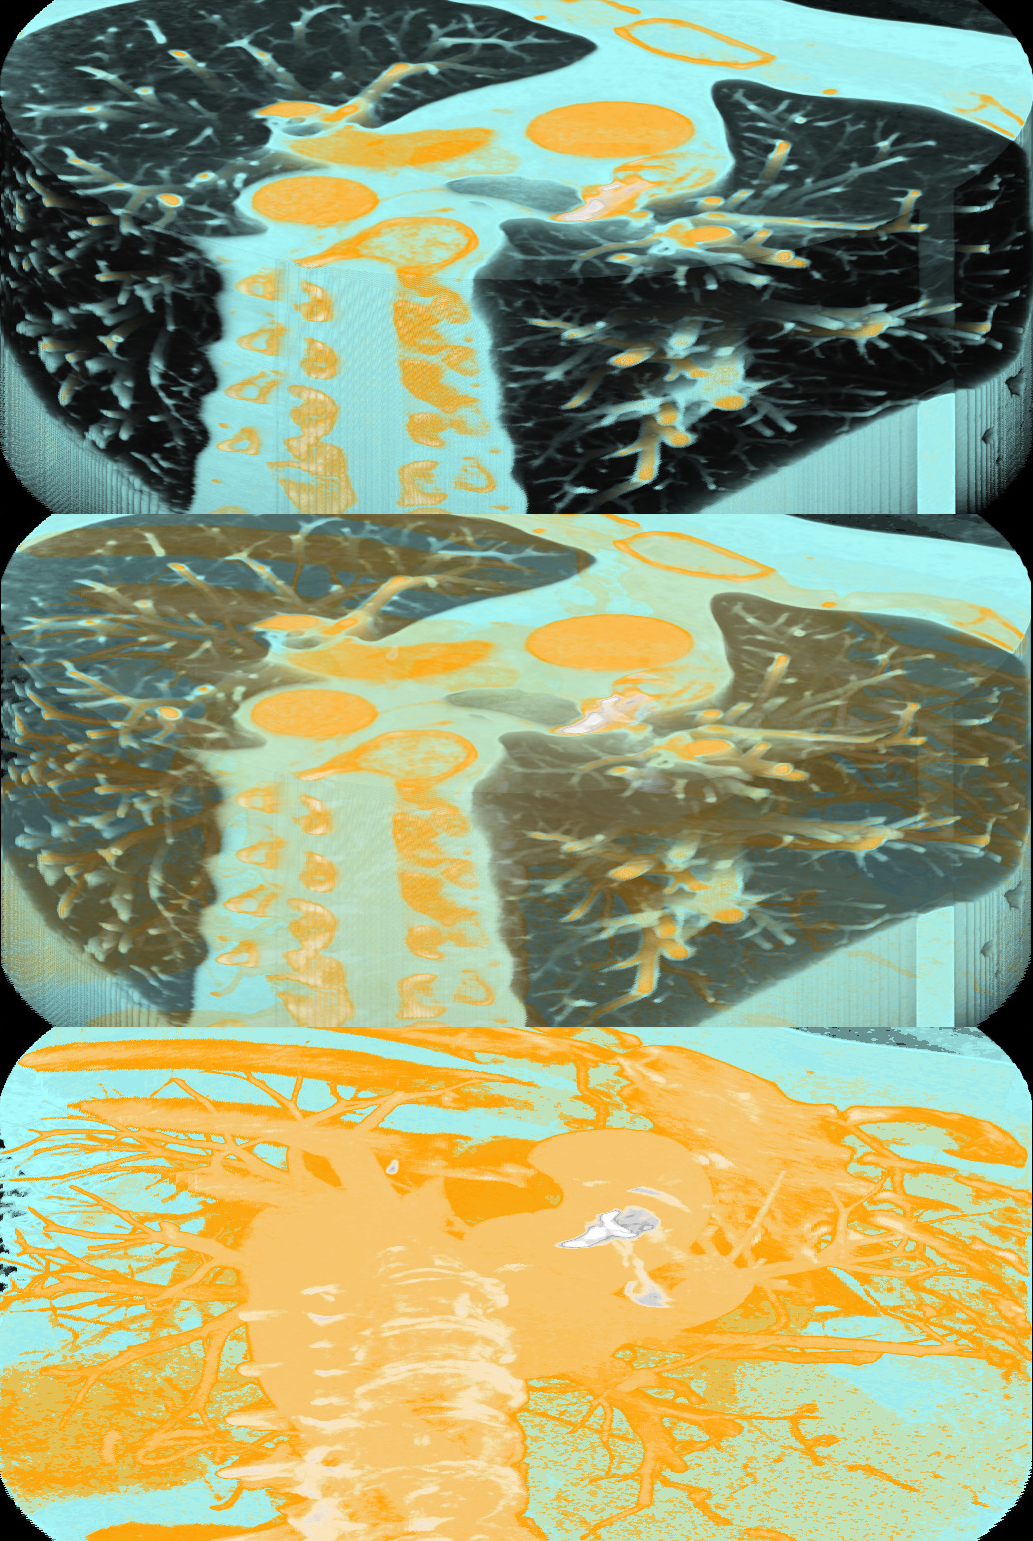
\includegraphics[width=0.35\textwidth]{MIDA_CARDIX_03.png} \\
	\caption{ \emph{CARDIX}\cite{gimias_sampledata_2018} dataset visualized with \emph{MIDA}. From top to bottom: DVR, MIDA, MIP.}
	\label{fig:MIDA_CARDIX_03}
\end{figure}


\begin{figure}[h]
	\centering
	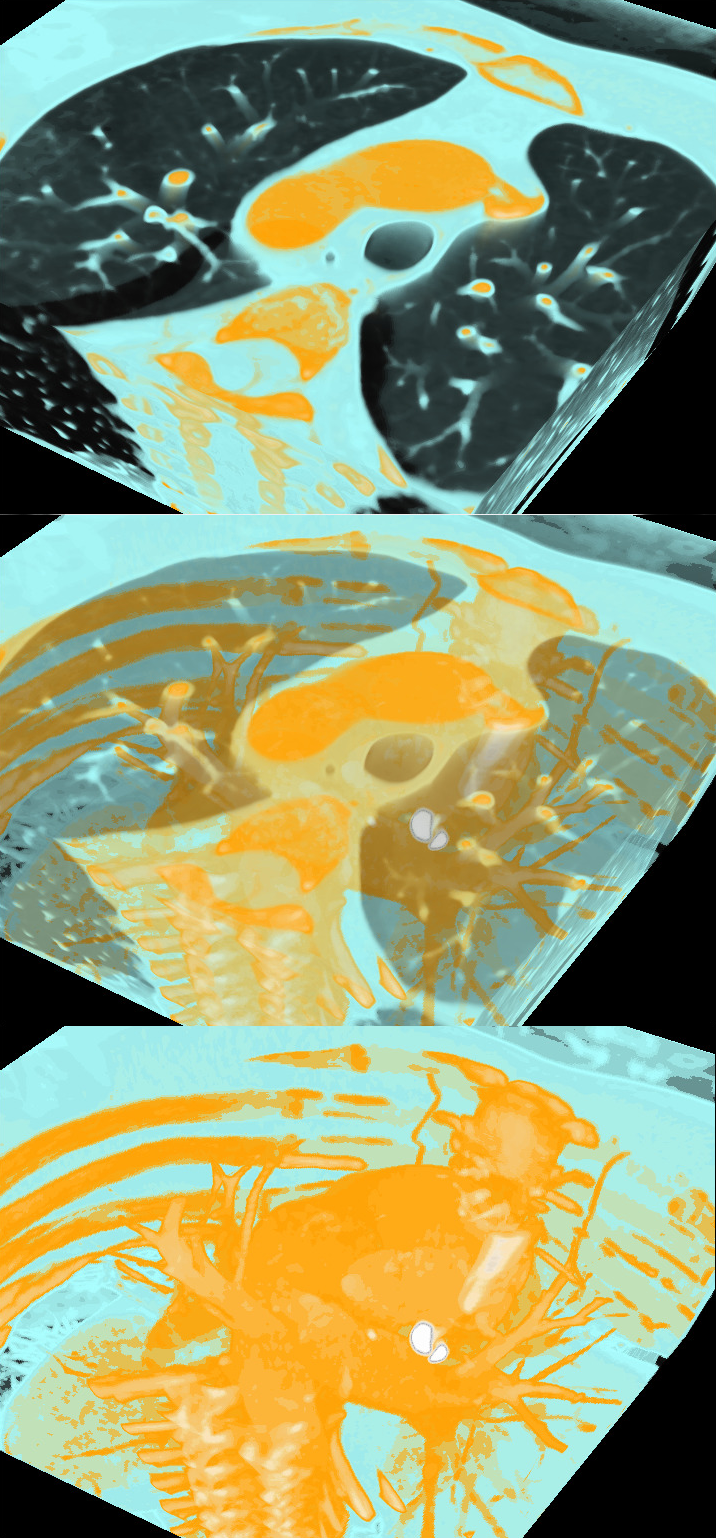
\includegraphics[width=0.35\textwidth]{MIDA_MAGIX_02.png} \\
	\caption{ \emph{MAGIX}\cite{gimias_sampledata_2018} dataset visualized with \emph{MIDA}. From top to bottom: DVR, MIDA, MIP.}
	\label{fig:MIDA_MAGIX_02}
\end{figure}

In figure \ref{fig:MIDA_CARDIX_03} and \ref{fig:MIDA_MAGIX_02} we can see the advantage of MIDA compared to DVR and MIP rendering. MIDA highlights important structures while not loosing a feeling of depth in the corresponding images.

\begin{figure}[h]
	\centering
	\includegraphics[width=0.45\textwidth]{MIDA_Angio_02.png} \\
	\caption{ \emph{Angio}\cite{gimias_sampledata_2018} dataset visualized with \emph{MIDA}. For each picture different transfer function settings are used.}
	\label{fig:MIDA_Angio_02}
\end{figure}

Figure \ref{fig:MIDA_Angio_02} shows several transfer function settings at the same MIDA-level. As seen certain coloring greatly enhance the visual perception of blood vessels and seperate them better from background information.
